\usetikzlibrary{automata,positioning,arrows}
\tikzset{
    ->, 
>=stealth, 
node distance=5cm,
every state/.style={thick, fill=gray!10},
initial text=$ $,}

\begin{figure}[H]
    \centering
    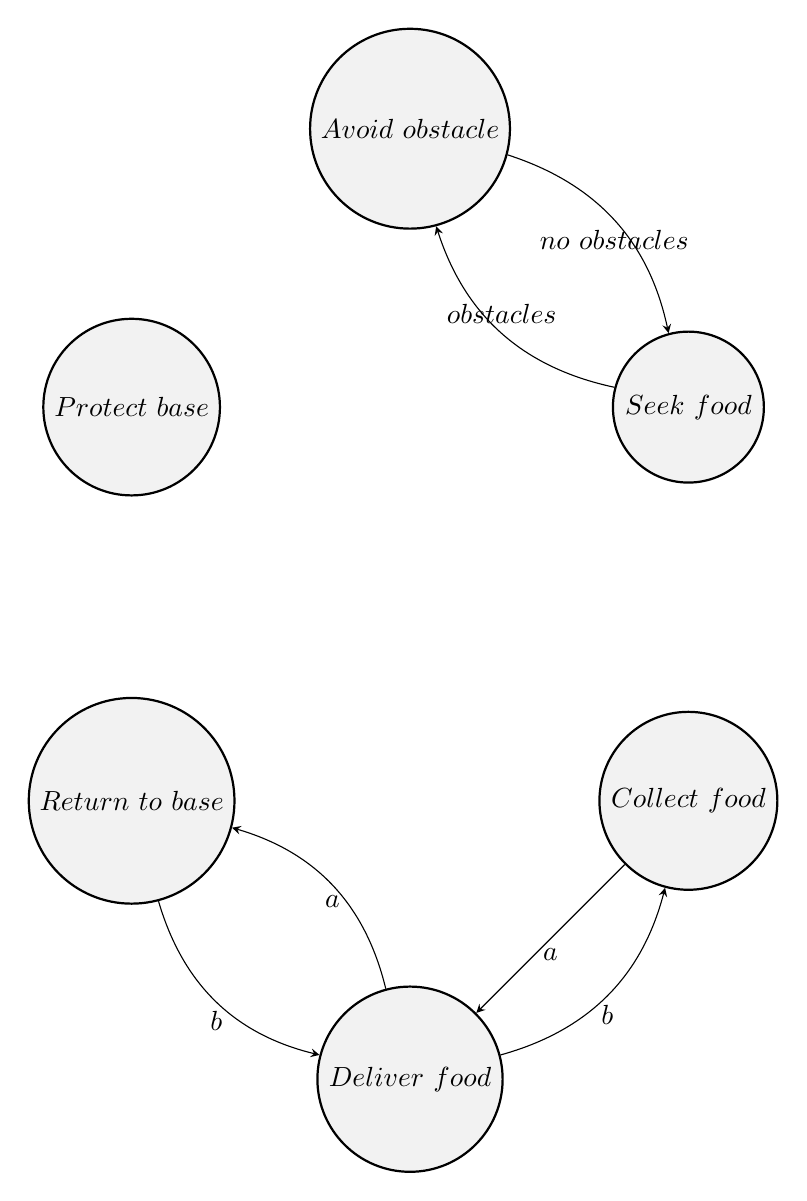
\begin{tikzpicture}
        \node[state] (1) {$Avoid\ obstacle$};
        \node[state, below left of=1] (2) {$Protect\ base$};
        \node[state, below right of=1] (3) {$Seek\ food$};
        \node[state, below of=3] (4) {$Collect\ food$};
        \node[state, below left of=4] (5) {$Deliver\ food$};
        \node[state, below of=2] (9) {$Return\ to\ base$};
        % \node[state, below  left of=1] (6) {$Flee\ enemy$};
        % \node[state, below  of=6] (7) {$Towards\ enemy$};
        % \node[state, below  of=7] (8) {$Attack\ enemy$};
        \draw
        (1) edge[below, bend left] node{$no\ obstacles$} (3)
        (3) edge[above, bend left] node{$obstacles$} (1)
        % (1) edge[below, bend right] node{$no\ obstacles$} (6)
        % (6) edge[above, bend right] node{$obstacles$} (1)
    
        (4) edge[below] node{$a$} (5)
        (5) edge[below, bend right] node{$b$} (4)
    
        (5) edge[below, bend right] node{$a$} (9)
        (9) edge[below, bend right] node{$b$} (5)
    
        ;
    \end{tikzpicture}
    \caption{Agent FSM}
    \label{fig:agent_FSM}
\end{figure}


